\documentclass[conference]{IEEEtran}
\usepackage{amsmath,amssymb}
\usepackage{booktabs}
\usepackage{flushend}
\usepackage{cite}
\usepackage{graphicx}
\usepackage{microtype}
\usepackage{subfig}
\usepackage[hidelinks]{hyperref}
\usepackage{url}

\hypersetup{
  pdftitle={Training Binary-Weight Diffusion Models from Scratch: A Controlled MNIST and CIFAR-10 Study},
  pdfauthor={Ayushman Bhattacharya, Anwesha Chakraborty, and Nihal Gazi},
  pdfkeywords={binary neural networks, diffusion models, quantization-aware training, post-training quantization}
}

\newcommand{\dfid}{\ensuremath{\mathrm{dFID}}}
\newcommand{\dkid}{\ensuremath{\mathrm{dKID}}}

\begin{document}

\title{Training Binary-Weight Diffusion Models from\\
Scratch: A Controlled MNIST and CIFAR-10 Study}

\author{
\IEEEauthorblockN{Ayushman Bhattacharya}
\IEEEauthorblockA{Pollinations AI\\ayushman.elixpo@gmail.com}
\and
\IEEEauthorblockN{Anwesha Chakraborty}
\IEEEauthorblockA{Dept. of CSE, JIS University\\anwesha.elixpo@gmail.com}
\and
\IEEEauthorblockN{Nihal Gazi}
\IEEEauthorblockA{Dept. of CSE (AI \& ML), IEM\\nihalg2006@gmail.com}
}

\maketitle

\begin{center}
\footnotesize\textit{Preprint \textbullet\ MonoDiffuse-TR-2026-01 \textbullet\ 14 Oct. 2026}
\end{center}
\vspace{-0.8em}

\begin{abstract}
At one bit per weight, post-training quantization (PTQ) can destroy a diffusion
model's denoising function. Does this imply that a useful binary score network
must be distilled from a floating-point teacher? We isolate that question in a
small residual U-Net whose parameterization is identical across precision
conditions. We compare FP32 training, zero-shot PTQ, binary-weight training from
random initialization, floating-point warm-started quantization-aware training
(QAT), and a binary-weight/binary-activation core. We additionally cross
mean-centering with pre- versus post-activation residual ordering. All conditions
use the same data, optimizer, per-stage budget, and ancestral 1,000-step DDPM
sampler and are repeated over three training seeds; warm QAT additionally
inherits a 12-epoch FP32 checkpoint. Evaluation uses a held-out
domain encoder and reports Fr\'echet and kernel distances, density, coverage, and
class-prior divergence, together with real--real and Gaussian-noise controls.
On MNIST, the best native W1A32 condition obtains domain-feature Fr\'echet distance
$46.33\mathbin{\pm}17.24$, far below zero-shot PTQ
($1314.20\mathbin{\pm}314.96$), but well above FP32
($3.15\mathbin{\pm}0.38$). On CIFAR-10, all conditions fail the control audit:
even FP32 obtains $382.67\mathbin{\pm}46.91$ versus a real--real baseline of
$7.13$. The previously proposed centering explanation is not
supported: centering increases latent-to-binary angular error and worsens the
pre-activation model. Thus, native optimization substantially mitigates PTQ
collapse on MNIST, but neither establishes parity with floating point nor
generalization to natural images.
We release code, per-seed checkpoints, hashes, histories, controls, and physically
bit-packed inference weights. Our conclusion is deliberately bounded: training
path matters at one bit, while a general teacher-free solution to binary diffusion
remains open.
\end{abstract}

\begin{IEEEkeywords}
binary neural networks, diffusion models, quantization-aware training,
post-training quantization, reproducibility
\end{IEEEkeywords}

\section{Introduction}

Diffusion models learn to reverse a gradual Gaussian corruption process and have
become a standard approach to image generation~\cite{ho2020ddpm}. Their repeated
denoising passes make model memory and arithmetic especially relevant on limited
hardware. Binary neural networks replace many floating-point weights with signs
and per-channel scales~\cite{hubara2016bnn,rastegari2016xnornet}. Such weights can
be stored compactly and can, with specialized kernels, admit binary arithmetic.
The latter qualification is important: binary-valued tensors in ordinary PyTorch
convolutions do not by themselves produce an XNOR speedup.

Recent diffusion quantization work has shown strong results at moderate bit
widths~\cite{li2023qdiffusion,he2023ptqd}. BiDM extends the question to binary
weights and activations, using a purpose-built structure and distillation from a
full-precision teacher~\cite{bidm2024}. Its observation that naive full
binarization is catastrophic motivates a narrower question: how much of that
failure follows from the binary representation, and how much follows from
projecting a floating-point solution into it after training?

We answer only at small scale. Rather than propose a new binary primitive, we
perform a controlled comparison of three training paths: zero-shot PTQ, native
training under binary forwards, and warm-started QAT. Parameter names, shapes,
biases, boundary layers, optimizer, and sampling are held fixed. We also test two
architectural explanations that appeared plausible in preliminary experiments:
per-filter mean-centering and pre-activation residual ordering. Finally, we audit
the evaluation itself. A classifier-confidence ``legibility'' score used in an
earlier draft gives a 100\% confidence floor on Gaussian noise and is therefore
removed as a quality metric.

The study makes four contributions:
\begin{itemize}
  \item a parameter-compatible comparison of FP32, native W1A32, PTQ W1A32,
  warm-started QAT, and a W1A1 core, each with three independent training seeds;
  \item a factorial MNIST ablation showing that pre-activation helps in the best
  native condition but mean-centering does not support the proposed geometric
  explanation;
  \item a calibrated distributional evaluation with real--real and noise controls,
  replacing an invalid confidence-based headline metric; and
  \item reproducible artifacts, including SHA-256 provenance and an actual packed
  binary-weight export whose whole-model payload is measured rather than inferred
  from the nominal bit width.
\end{itemize}

The result is a correction as much as a positive finding. Native W1A32 training
is much more effective than zero-shot PTQ on MNIST, yet remains clearly behind the
matched FP32 model. We therefore do not claim floating-point parity, a theorem
about centering, or measured runtime/energy gains.

\section{Related Work}

\paragraph{Diffusion.}
A DDPM trains a time-conditioned network to predict noise added to a clean sample
and samples through a Markov reverse process~\cite{ho2020ddpm}. DDIM provides a
non-Markovian alternative sampler~\cite{song2020ddim}; improved objectives and
parameterizations can further raise quality~\cite{nichol2021improved}. We retain
the original noise-prediction objective and ancestral sampler to minimize moving
parts.

\paragraph{Quantized diffusion.}
Q-Diffusion and PTQD address the unusual activation distributions and error
accumulation of diffusion PTQ at 4--8 bits
~\cite{li2023qdiffusion,he2023ptqd}. BinaryDM uses quantization-aware training,
evolvable binary bases, and representation mimicking for W1A4 diffusion
~\cite{binarydm2025}. BiDM studies binary weights and activations with a
timestep-friendly architecture and spatially patched distillation
~\cite{bidm2024}. Our tiny unconditional networks are not competitors to these
large-scale systems. They instead isolate initialization and training path while
holding the model topology constant.

\paragraph{Binary networks.}
BinaryConnect and subsequent BNN work train latent real-valued parameters while
using sign-projected weights during forward passes
~\cite{courbariaux2015binaryconnect,hubara2016bnn}. XNOR-Net introduced magnitude
scales that approximate real filters~\cite{rastegari2016xnornet}. Gradients
through discontinuous signs are commonly approximated by straight-through
estimators (STEs)~\cite{bengio2013ste}. These established components form our
binary layers; novelty is not claimed for the optimizer or quantizer.

\section{Controlled Study Design}

\subsection{Objective and model}

For clean image $x_0$, Gaussian noise $\epsilon$, and timestep $t$, all models
minimize
\begin{equation}
\mathcal{L}=\mathbb{E}_{x_0,t,\epsilon}
\left\|\epsilon-\epsilon_\theta
\left(\sqrt{\bar\alpha_t}x_0+
\sqrt{1-\bar\alpha_t}\epsilon,t\right)\right\|_2^2.
\end{equation}
We use 1,000 linearly spaced diffusion steps. The denoiser is a compact residual
U-Net~\cite{ronneberger2015unet} with base width 16, widths $[16,32,64]$, two
downsampling stages, two skip concatenations, sinusoidal time
embeddings~\cite{vaswani2017attention}, and GroupNorm. It has 218,993
parameters on MNIST. Input/output convolutions, normalization, time-conditioning
linears, biases, scales, and residual additions remain FP32 in every condition.
Consequently, ``W1A1 core'' is more accurate than ``fully binary network.''

\subsection{Binary forward pass}

For output filter $W_o$, uncentered projection uses
\begin{equation}
\widehat W_o=\alpha_o\operatorname{sign}(W_o),\qquad
\alpha_o=\operatorname{mean}(|W_o|).
\end{equation}
The centered variant replaces $W_o$ by $W_o-\mu_o$, where
$\mu_o=\operatorname{mean}(W_o)$, before computing both sign and scale. Latent
FP32 parameters are updated with an identity STE. In the W1A1 core, block
activations additionally use a sign forward and clipped-identity backward pass.
Boundary layers stay floating point to avoid discretizing pixels and predicted
noise.

\subsection{Conditions}

Table~\ref{tab:conditions} defines the interventions. ``Native'' means random
initialization with binary weights used from the first forward pass. PTQ loads a
converged FP32 state dictionary and changes only the forward projection, with no
calibration or retraining. Warm QAT loads that same FP32 checkpoint and trains for
the full binary budget. PTQ here is intentionally a zero-shot stress test, not a
comparison against sophisticated diffusion PTQ methods.

\begin{table}[t]
\centering
\caption{Controlled conditions. Activations are FP32 unless marked binary.}
\label{tab:conditions}
\small
\begin{tabular}{lll}
\toprule
Condition & Initialization & Core precision \\
\midrule
FP32 & random & W32/A32 \\
Native W1A32 & random & W1/A32 \\
PTQ W1A32 & FP32 final & W1/A32 \\
Warm QAT W1A32 & FP32 final & W1/A32 \\
Native W1A1 core & random & W1/A1 \\
\bottomrule
\end{tabular}
\end{table}

For native W1A32 on MNIST we cross centered/uncentered projection with pre- and
post-activation residual blocks~\cite{he2016preact}. All variants have identical
trainable parameter counts and compatible state dictionaries.

\subsection{Data and optimization}

We use the canonical 60,000/10,000 MNIST split~\cite{lecun1998mnist} and the
50,000/10,000 CIFAR-10 split~\cite{krizhevsky2009cifar}. Images are scaled to
$[-1,1]$; CIFAR-10 training uses random crop and horizontal flip. Each condition
is optimized in 12-epoch stages with AdamW~\cite{loshchilov2019adamw}, learning
rate $2\times10^{-4}$, weight decay $10^{-4}$, cosine decay, gradient norm
clipping at 1, batch size 256 for MNIST and 128 for CIFAR-10, and seeds
$\{0,1,2\}$. AMP accelerates training, while stored parameters and evaluation
remain FP32. The sampler is ancestral DDPM with all 1,000 reverse steps. Each
reported model distribution uses 2,000 samples from a fixed sampling seed; the
training seed changes independently.

Native and FP32 models receive one optimization stage. PTQ adds no training after
the FP32 stage, whereas warm QAT receives a second 12-epoch stage after loading
FP32. Thus warm QAT uses 24 total training epochs; its initialization is not
treated as free compute.

\subsection{Evaluation and controls}

An independently initialized domain classifier is trained only on the real
training split. Its penultimate features define domain-feature Fr\'echet distance
(\dfid)~\cite{heusel2017fid}, unbiased cubic-polynomial kernel distance (\dkid)
~\cite{binkowski2018kid}, and $k=5$ density and coverage
~\cite{naeem2020density}. We also report Jensen--Shannon divergence between mean
predicted class distributions. Lower is better for \dfid, \dkid, and JS; higher
is better for density and coverage. These are domain-feature metrics, not
ImageNet Inception FID, and should not be compared numerically with standard FID
leaderboards.

The MNIST encoder reaches 98.03\% test accuracy and 1.44\% ten-bin expected
calibration error. A disjoint real--real split gives \dfid{} 0.076, density
0.969, and coverage 0.971. Clamped Gaussian noise gives \dfid{} 2278.24 and zero
density/coverage. Yet the same noise receives mean peak classifier confidence
1.000, demonstrating why confidence is retained only as a diagnostic and not as a
quality score.

The independently trained CIFAR-10 encoder reaches 91.51\% test accuracy and
4.48\% expected calibration error. Its real--real control gives \dfid{} 7.13,
\dkid{} 0.002, density 1.013, and coverage 0.969; clamped Gaussian noise gives
\dfid{} 607.86, \dkid{} 4.668, density 0.008, and coverage 0.001. These controls
make the poor absolute performance of the compact CIFAR-10 generators visible.

\section{MNIST Results}

\begin{table*}[t]
\centering
\caption{MNIST distribution metrics, mean $\pm$ sample standard deviation over
three training seeds. All models use the same 2,000-sample ancestral-DDPM
evaluation. Best non-FP result in bold.}
\label{tab:mnist}
\small
\begin{tabular}{lrrrrr}
\toprule
Condition & \dfid{} $\downarrow$ & \dkid{} $\downarrow$ & Density $\uparrow$ & Coverage $\uparrow$ & Class JS $\downarrow$ \\
\midrule
FP32 & $3.15\pm0.38$ & $0.056\pm0.013$ & $0.284\pm0.014$ & $0.195\pm0.017$ & $0.033\pm0.009$ \\
Native, uncentered, pre & $\mathbf{46.33\pm17.24}$ & $\mathbf{1.286\pm0.816}$ & $0.022\pm0.005$ & $\mathbf{0.033\pm0.010}$ & $0.295\pm0.020$ \\
Native, centered, pre & $99.50\pm25.77$ & $7.598\pm3.223$ & $0.010\pm0.008$ & $0.017\pm0.014$ & $0.308\pm0.047$ \\
Native, uncentered, post & $84.26\pm61.39$ & $6.881\pm6.897$ & $0.033\pm0.051$ & $0.028\pm0.034$ & $0.286\pm0.113$ \\
Native, centered, post & $82.46\pm61.39$ & $7.943\pm8.043$ & $\mathbf{0.037\pm0.043}$ & $0.032\pm0.025$ & $\mathbf{0.253\pm0.087}$ \\
Warm QAT, centered, pre & $66.45\pm28.49$ & $4.945\pm3.686$ & $0.019\pm0.004$ & $0.032\pm0.004$ & $0.320\pm0.059$ \\
Native W1A1 core & $204.55\pm69.77$ & $41.03\pm25.01$ & $0.005\pm0.002$ & $0.009\pm0.004$ & $0.339\pm0.027$ \\
PTQ, centered, pre & $871.12\pm717.34$ & $1581.31\pm2433.16$ & $0$ & $0$ & $0.533\pm0.000$ \\
PTQ, uncentered, pre & $1314.20\pm314.96$ & $2467.50\pm1549.51$ & $0$ & $0$ & $0.531\pm0.002$ \\
\bottomrule
\end{tabular}
\end{table*}

\subsection{Native training mitigates PTQ collapse, without FP parity}

Table~\ref{tab:mnist} gives the central result. The best native W1A32 condition
reduces \dfid{} from $1314.20$ under matched uncentered PTQ to $46.33$. Its
nonzero density and coverage also show that the gain is not solely a shift in the
first two feature moments. Nevertheless, FP32 is substantially better on every
distributional metric. The defensible conclusion is therefore not ``binary
matches floating point,'' but ``the training path accounts for a large fraction
of zero-shot one-bit PTQ failure on MNIST.''

Warm-started centered QAT improves upon centered native training in \dfid{}
($66.45$ versus $99.50$), so a floating-point initialization is not intrinsically
harmful once binary forwards are optimized. Native training's advantage is over
zero-shot projection, not over every teacher- or warm-start-dependent method.

\subsection{The centering hypothesis is rejected}

Centering moves the mean positive-sign fraction closer to 0.5, but this balance
does not imply better filter geometry or generation. Averaged over seeds,
centered pre-activation weights have $34.05^\circ$ latent-to-projected angular
error versus $33.29^\circ$ without centering. Corresponding \dfid{} worsens from
$46.33$ to $99.50$. Under post-activation the \dfid{} means are similar and have
large seed variance, while \dkid{} is worse with centering. These observations
directly contradict the earlier ``structural dominance'' account; we discard it
rather than relabel the heuristic as theory.

Pre-activation is useful only conditionally. It improves the uncentered mean from
\dfid{} $84.26$ to $46.33$, but not the centered mean. This interaction and the
large three-seed variance argue against presenting residual ordering as a general
stability principle.

\subsection{Activation binarization remains difficult}

The W1A1 core is trained natively yet degrades to \dfid{}
$204.55\mathbin{\pm}69.77$. It remains better than zero-shot PTQ in \dfid{}, but
its very low density and coverage indicate a large distributional gap. Moreover,
the model is not end-to-end binary because boundaries, normalization, time
conditioning, scales, and accumulation remain floating point.

\begin{figure}[t]
\centering
\subfloat[FP32]{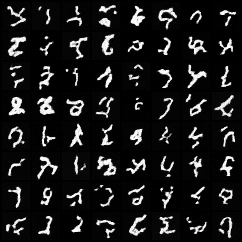
\includegraphics[width=.31\columnwidth]{figures/results/mnist-fp.png}}\hfill
\subfloat[Native W1A32]{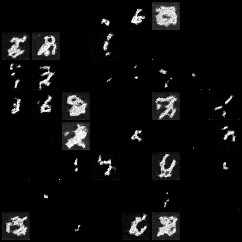
\includegraphics[width=.31\columnwidth]{figures/results/mnist-native-w1a32.png}}\hfill
\subfloat[PTQ W1A32]{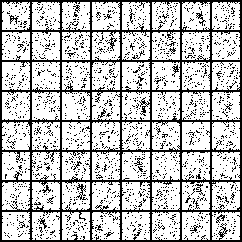
\includegraphics[width=.31\columnwidth]{figures/results/mnist-ptq-w1a32.png}}
\caption{MNIST samples from the fixed evaluation seed. The native binary model
retains digit-like structure but is visibly below FP32; zero-shot PTQ collapses.}
\label{fig:mnist}
\end{figure}

\subsection{Storage accounting}

Binary convolutions contain 195,328 of 218,993 parameters (89.19\%). A physical
export packs their signs with \texttt{numpy.packbits}, stores one FP32 scale per
output channel, and retains all non-binary tensors as FP32. The resulting tensor
payload is 121,316 bytes versus 875,972 bytes for an all-FP32 state, a 7.22$\times$
whole-model reduction; the self-describing NPZ container is 143,350 bytes. This
is smaller than the often-quoted 32$\times$ figure because 10.81\% of parameters,
normalization state, and scales are not binary. It is a storage measurement, not
a runtime or energy measurement.

\section{CIFAR-10 Stress Test}

The same base-width-16 model and 12-epoch budget are applied to CIFAR-10 without
architecture tuning. We evaluate FP32, centered and uncentered native W1A32,
centered PTQ, centered warm QAT, and the W1A1 core over three seeds. This is a
natural-image stress test of the MNIST observation, not a competitive CIFAR-10
generator.

\begin{table*}[t]
\centering
\caption{CIFAR-10 stress test, mean $\pm$ sample standard deviation over three
training seeds. The real--real control has \dfid{} 7.13, \dkid{} 0.002, density
1.013, and coverage 0.969. Bold marks the best model mean, not a claim of success.}
\label{tab:cifar}
\small
\begin{tabular}{lrrrrr}
\toprule
Condition & \dfid{} $\downarrow$ & \dkid{} $\downarrow$ & Density $\uparrow$ & Coverage $\uparrow$ & Class JS $\downarrow$ \\
\midrule
FP32 & $382.67\pm46.91$ & $3.094\pm0.353$ & $0.230\pm0.132$ & $0.082\pm0.046$ & $0.146\pm0.031$ \\
Native, uncentered, pre & $402.46\pm21.56$ & $3.454\pm0.347$ & $0.125\pm0.023$ & $0.048\pm0.005$ & $\mathbf{0.143\pm0.010}$ \\
Native, centered, pre & $384.32\pm11.95$ & $3.244\pm0.136$ & $0.183\pm0.086$ & $0.061\pm0.011$ & $0.168\pm0.003$ \\
Warm QAT, centered, pre & $403.61\pm22.46$ & $3.301\pm0.194$ & $0.155\pm0.065$ & $0.056\pm0.022$ & $0.180\pm0.017$ \\
Native W1A1 core & $\mathbf{365.02\pm26.97}$ & $\mathbf{3.078\pm0.237}$ & $\mathbf{0.293\pm0.105}$ & $\mathbf{0.082\pm0.014}$ & $0.152\pm0.019$ \\
PTQ, centered, pre & $564.21\pm36.08$ & $4.377\pm0.282$ & $0.059\pm0.023$ & $0.003\pm0.001$ & $0.262\pm0.058$ \\
\bottomrule
\end{tabular}
\end{table*}

Native optimization again avoids the worst zero-shot PTQ collapse. However, the
FP32 model itself is hundreds of \dfid{} points from the real--real control and
has only 0.082 coverage. Although the W1A1 core has the best mean \dfid{}, \dkid{},
density, and coverage among these weak generators, its three-seed intervals
overlap FP32 and its samples remain coarse (Fig.~\ref{fig:cifar}). The experiment
therefore cannot adjudicate binary-versus-FP quality on natural images; it shows
that this small architecture and budget are inadequate for that claim.

\begin{figure}[t]
\centering
\subfloat[FP32]{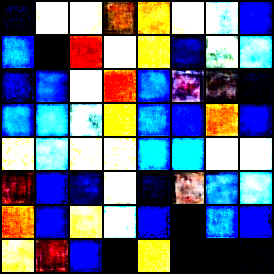
\includegraphics[width=.23\columnwidth]{figures/results/cifar10-fp.png}}\hfill
\subfloat[Native W1A32]{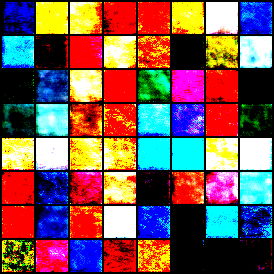
\includegraphics[width=.23\columnwidth]{figures/results/cifar10-native-w1a32.png}}\hfill
\subfloat[W1A1 core]{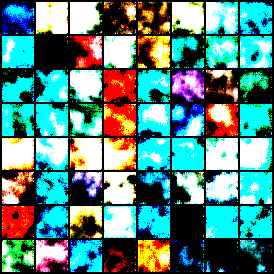
\includegraphics[width=.23\columnwidth]{figures/results/cifar10-native-w1a1.png}}\hfill
\subfloat[PTQ W1A32]{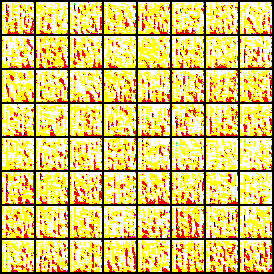
\includegraphics[width=.23\columnwidth]{figures/results/cifar10-ptq-w1a32.png}}
\caption{CIFAR-10 samples from seed 0. Even FP32 produces coarse color blocks;
the stress test is consequently not evidence of natural-image fidelity.}
\label{fig:cifar}
\end{figure}

\section{Discussion}

\paragraph{What the experiment supports.}
On MNIST, optimizing with the binary forward model is decisively better than
zero-shot sign projection. This is consistent with the binary and floating-point
objectives favoring different parameter regions. It does not establish that
random initialization is uniquely necessary: warm-started QAT also recovers much
of the PTQ loss. CIFAR-10 preserves the qualitative PTQ failure, but its failed
FP32 control prevents a stronger precision comparison.

\paragraph{What it falsifies.}
The experiments do not support FP parity, a centering theorem, a universally
superior pre-activation topology, or the validity of peak classifier confidence as
a generative quality metric. Correcting those points narrows the claim but makes
it testable.

\paragraph{Relation to BiDM.}
BiDM addresses W1A1 diffusion at substantially greater resolution and uses
specialized architecture and distillation~\cite{bidm2024}. Our results neither
replace nor directly compare with that system. They show, in a matched tiny
network, that zero-shot PTQ is an overly weak baseline for deciding whether binary
weights can be trained. Scaling teacher-free binary diffusion remains unresolved.

\section{Hardware Artifact: Diffuino}

As a system demonstration separate from the controlled study, we deploy
Diffuino on an Arduino UNO Q. The Qualcomm Linux processor executes a
class-conditioned MNIST diffusion model with ONNX Runtime and streams selected
states from the 1,000-step ancestral reverse process over Bridge RPC. The STM32
coprocessor refreshes the onboard $8\times13$ LED matrix, where each $28\times28$
state is rendered as a centered $8\times8$ grayscale digit. Four RGB LEDs report
CPU load, memory load, denoising progress, and agreement between the requested
class and a diagnostic classifier.

For a reliable interactive exhibit, the default artifact uses a separately
trained class-conditioned FP32 checkpoint. Fixed per-class sampling seeds and
display-only resize/contrast settings improve repeatable legibility on the small
matrix; neither is used in the paper's distributional evaluation. The study's
native W1A32 seed-2 checkpoint can also be exported to ONNX by materializing its
sign-scale convolution weights as ordinary floating-point convolution tensors.
Consequently, that path preserves the learned binary-weight representation but
does not execute packed XNOR convolutions. Diffuino therefore demonstrates
functional edge deployment and live diffusion visualization, not binary
arithmetic acceleration, latency reduction, or energy savings. The installable
app, packaging script, model files, and firmware are included with the released
code.

The exhibit accepts a decimal class from a four-switch BCD selector on STM32
pins D2--D5. Before a debounced generate pulse reaches D6, external logic checks
$\mathrm{VALID}=\neg[b_3\wedge(b_2\vee b_1)]$, so codes 10--15 are rejected in
hardware; firmware retains an independent range check. During sampling, further
triggers are ignored and the selected value is latched. The generated digit
remains on the display until a separate debounced D7 reset returns the system to
its ready state. The released KiCad design adds RC filtering, per-input series
protection, buffered indication, and local supply decoupling to the demonstrated
breadboard circuit. This human interface does not alter the sampler or any
reported metric.

\IfFileExists{figures/diffuino/diffuino-board.jpg}{
\IfFileExists{figures/diffuino/diffuino-board-2.jpg}{
\IfFileExists{figures/diffuino/diffuino-selector.png}{
\begin{figure*}[t]
\centering
\subfloat[Physical prototype: wider setup view (top) and LED-matrix close-up
(bottom).]{%
  \begin{minipage}[b]{0.32\textwidth}
  \centering
  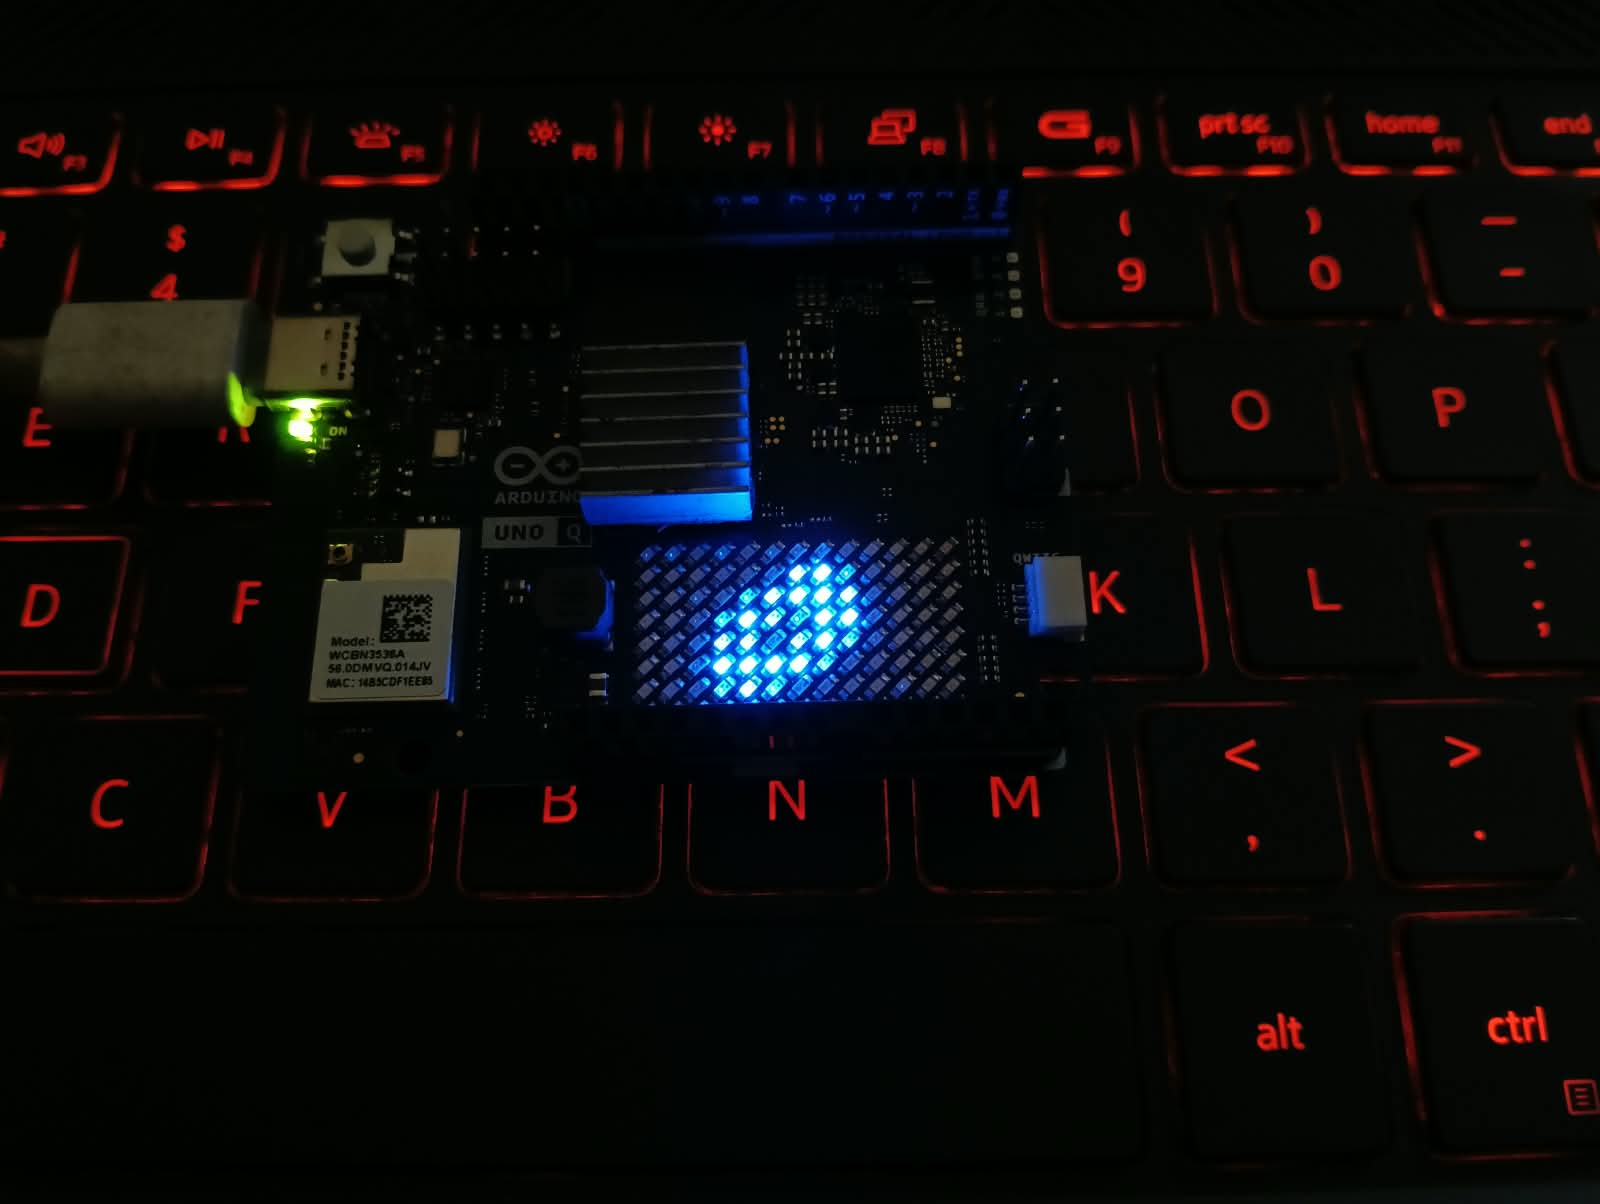
\includegraphics[width=\linewidth]{figures/diffuino/diffuino-board-2.jpg}\\[0.5ex]
  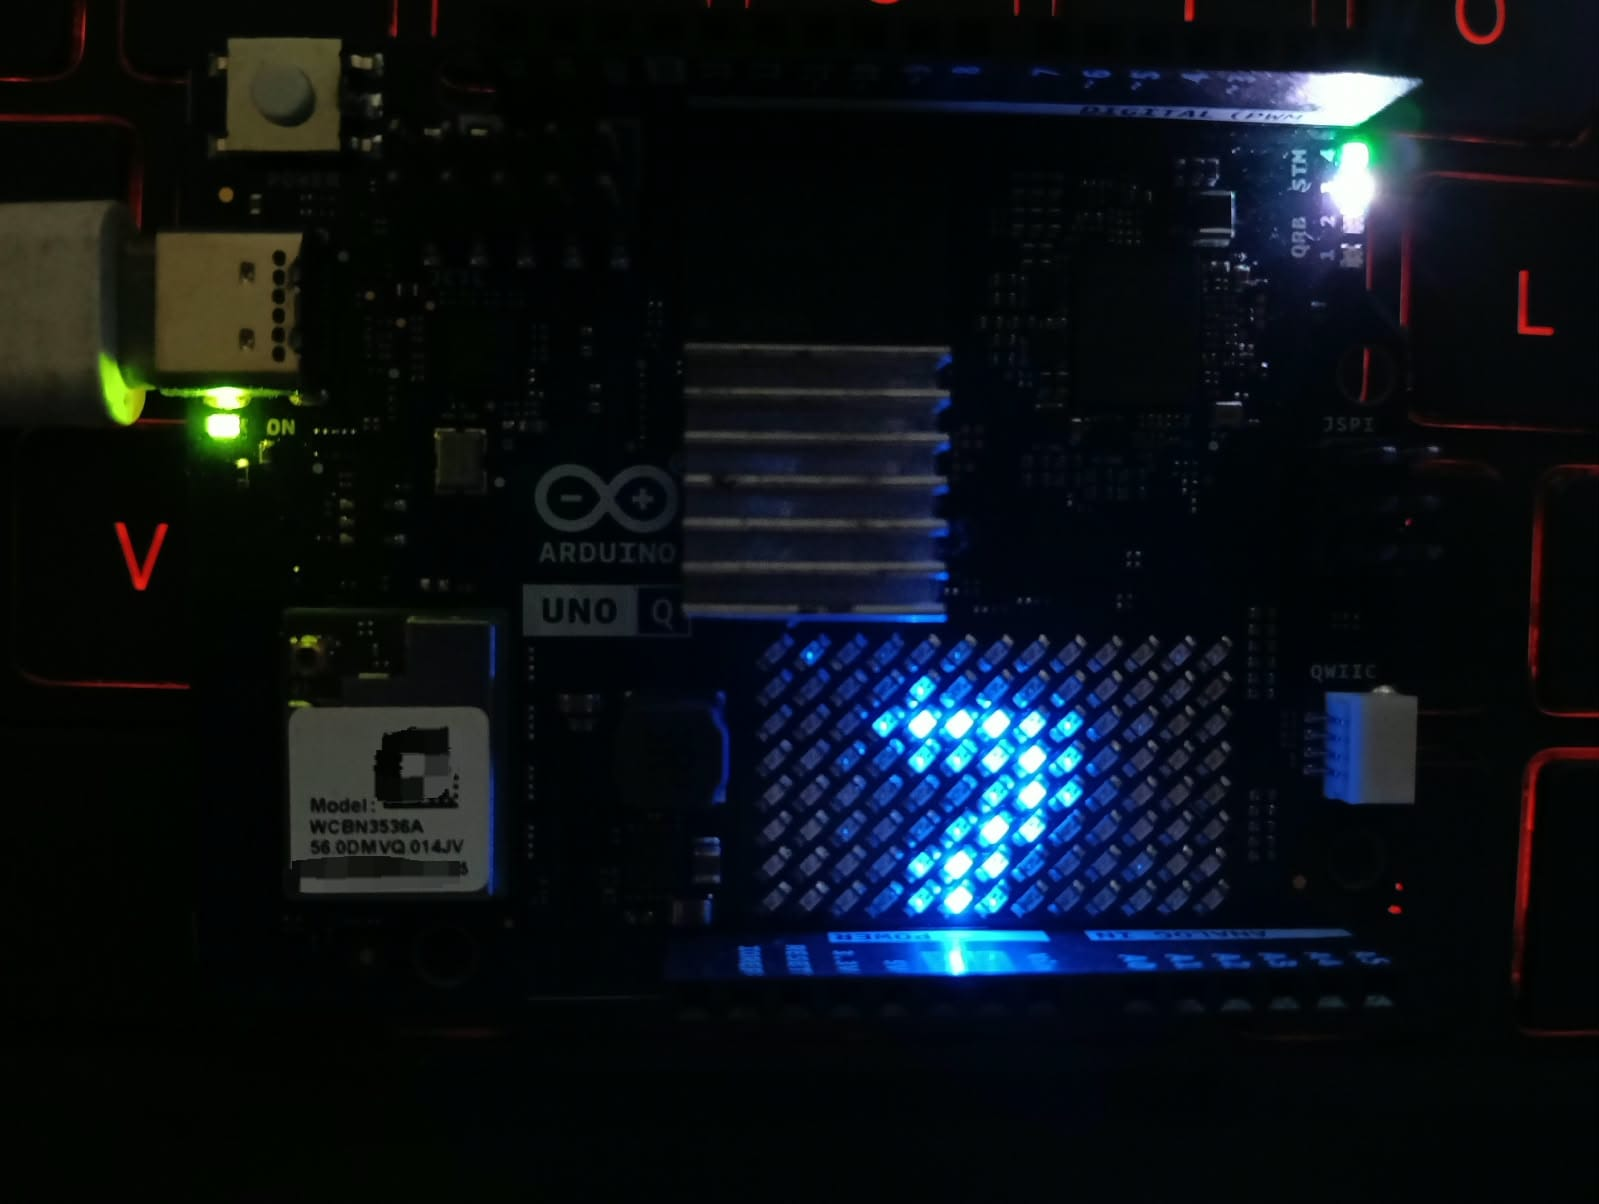
\includegraphics[width=\linewidth]{figures/diffuino/diffuino-board.jpg}
  \end{minipage}}
\hfill
\subfloat[Complete BCD selector and validity-interlock schematic.]{%
  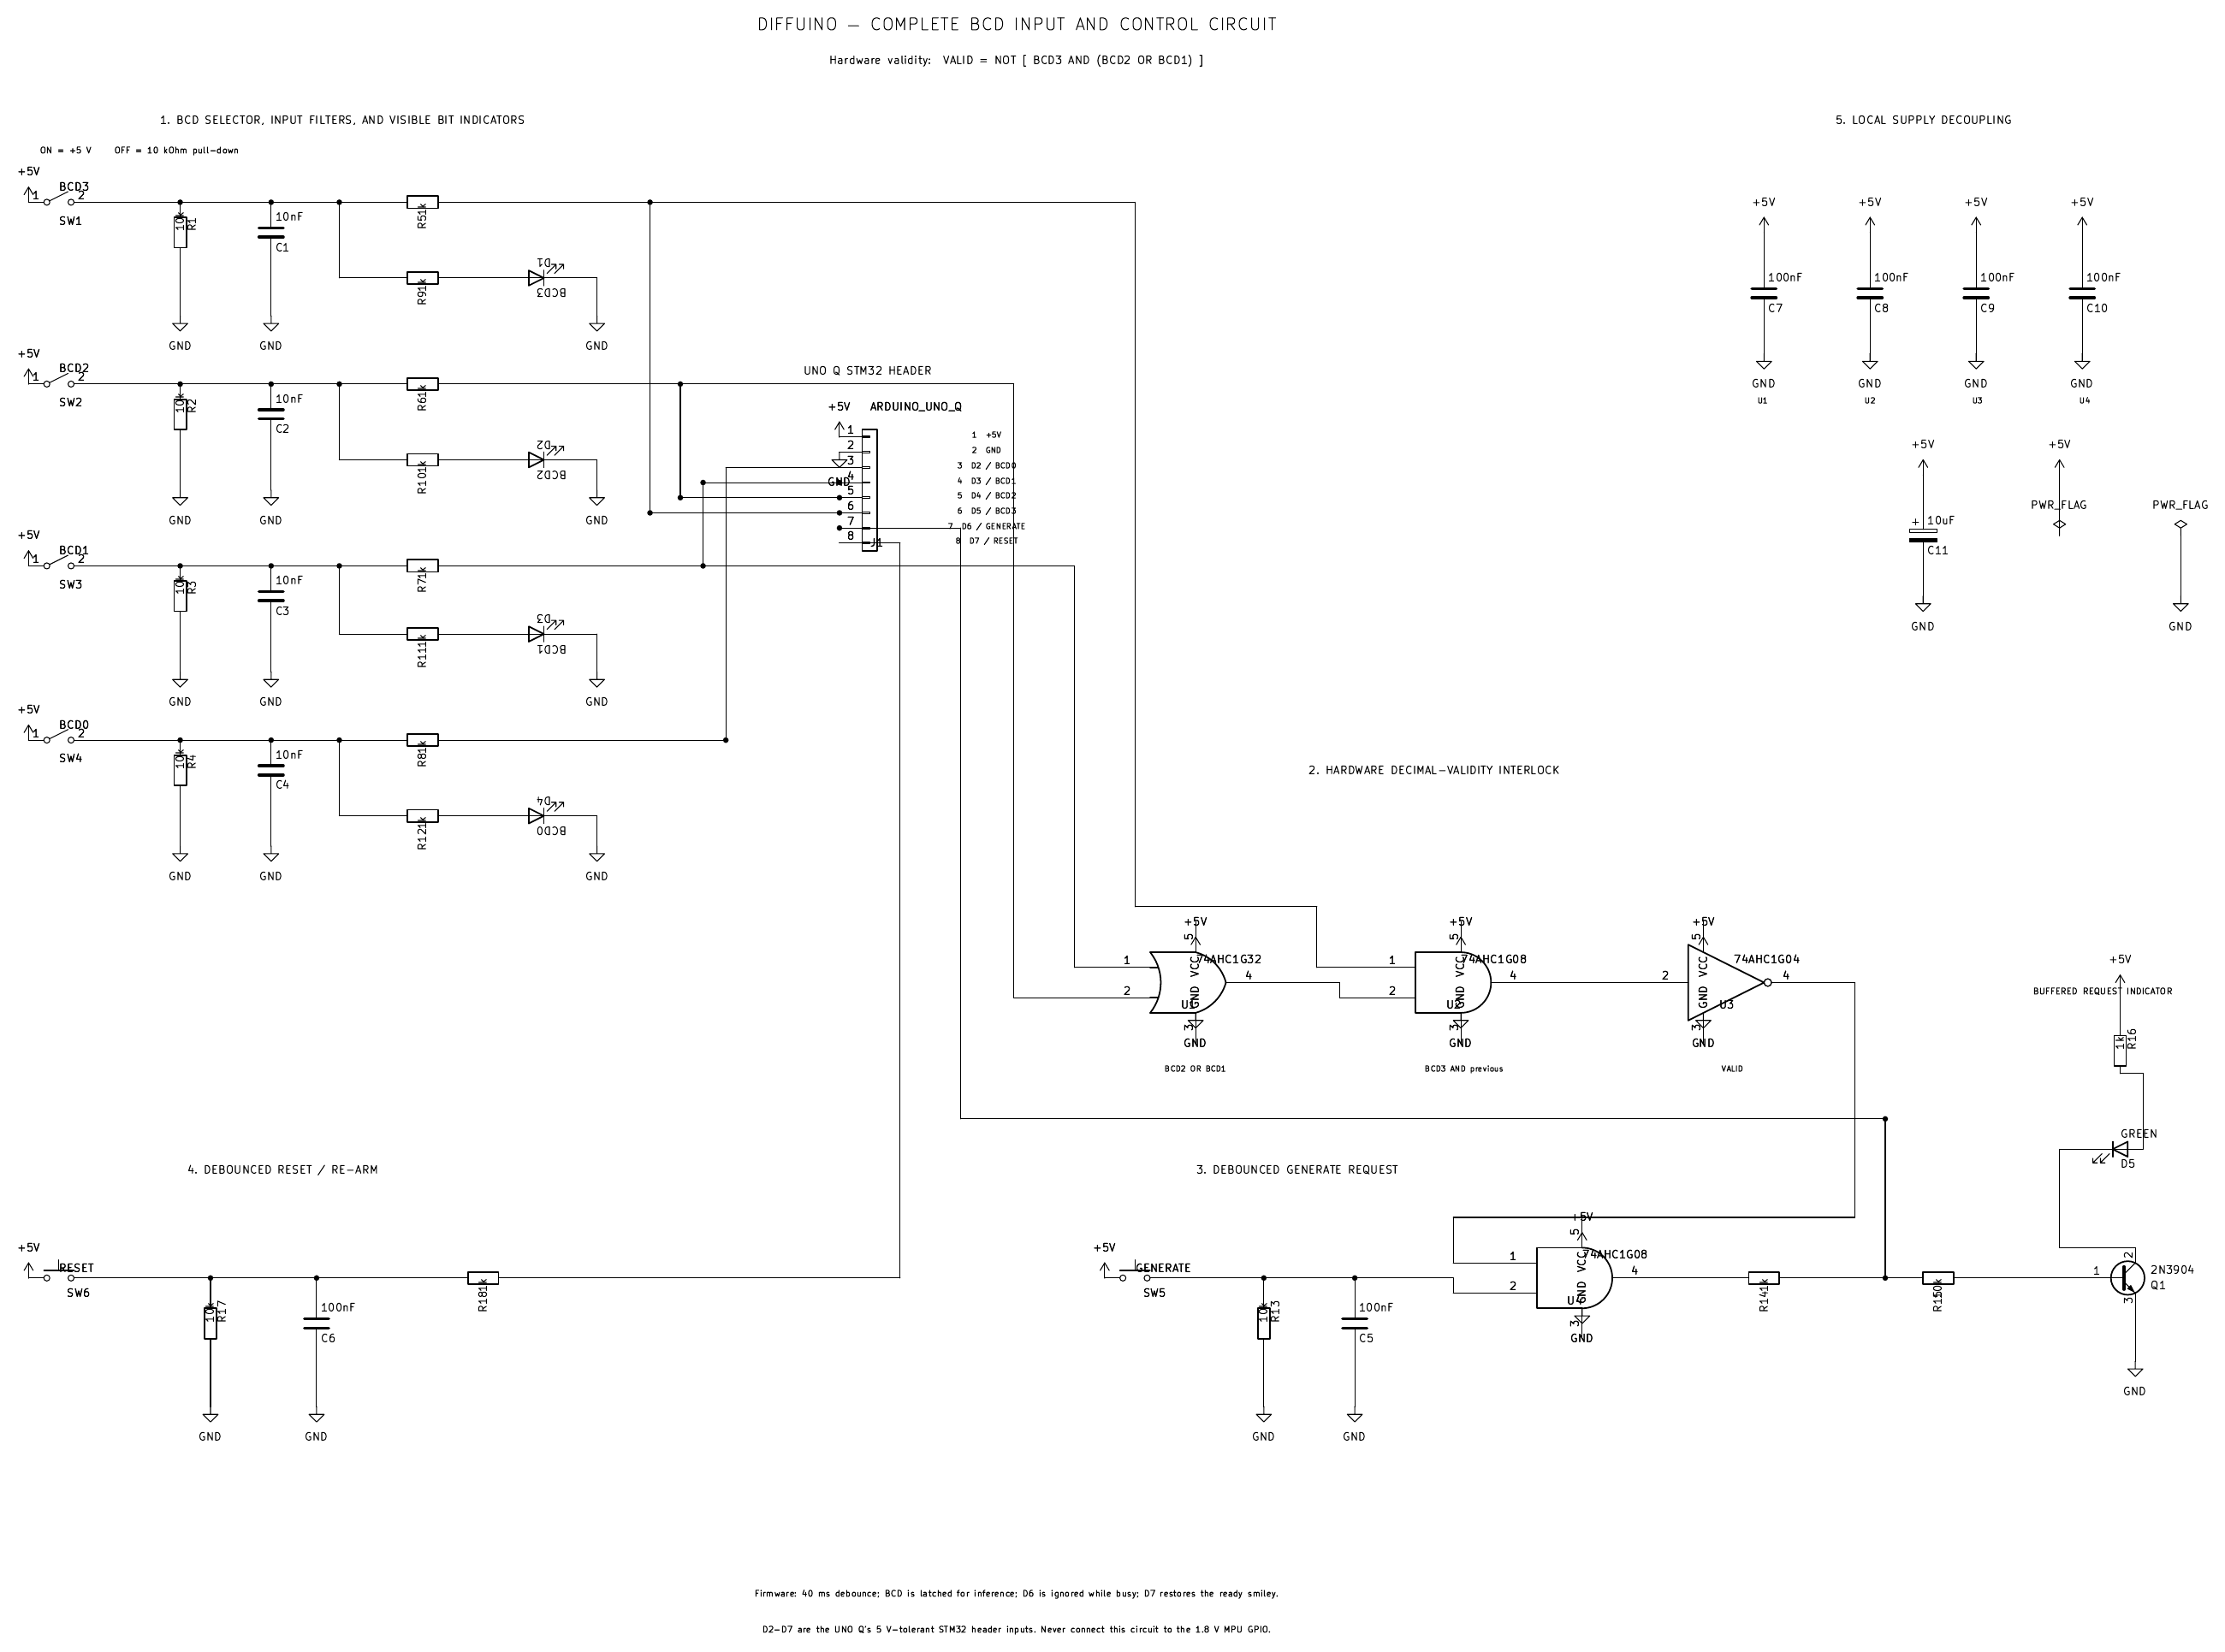
\includegraphics[width=0.65\textwidth]{figures/diffuino/diffuino-selector.png}}
\caption{Diffuino hardware artifact. The Qualcomm processor performs ONNX
inference while the STM32 drives the $8\times13$ matrix and status LEDs. Four
BCD inputs connect to D2--D5; the combinational interlock suppresses invalid
decimal codes before the generate request reaches D6, and D7 independently
re-arms the appliance. This artifact is separate from the controlled-study
metrics.}
\label{fig:diffuino}
\end{figure*}
}{}
}{}
}{}

\section{Limitations}

The network and training budget are intentionally small. Three seeds reveal large
variance but are insufficient for fine-grained significance claims. Each metric
uses 2,000 generated samples, so absolute estimates are noisier than common
50,000-sample evaluations. Domain encoders make the metrics meaningful for
digits, but their values are not comparable to standard ImageNet Inception FID.
Classifier features can also miss perceptual defects, which is why sample grids
and multiple density/diversity statistics are retained. The CIFAR-10 experiment
is a failed small-model stress test rather than a tuned benchmark; apparent
rankings within that low-quality regime should not be interpreted as
natural-image progress. Finally, storage is physically
packed, but no binary convolution kernel is implemented; latency, operation, and
energy improvements remain unmeasured.

\section{Reproducibility}

The released pipeline records configuration, per-epoch loss, training and sampling
seeds, package/CUDA/device versions, source commit, checkpoint SHA-256, parameter
accounting, and quantization diagnostics beside every checkpoint. Atomic JSON
writes prevent partial metadata. Evaluation artifacts include per-seed metrics,
aggregate means and sample standard deviations, encoder accuracy/calibration,
real--real and Gaussian-noise controls, and fixed-seed sample grids. Unit tests
cover parameter compatibility, forward shapes, diffusion schedules,
distribution-metric controls, and physical bit packing. The exact entry points
are documented in the released repository~\cite{monodiffuseRepo} under
\path{experiments/v1_binary_study}; all paper tables are traceable to
\path{artifacts/v1_binary_study}. Diffuino is distributed as a deterministically
generated Arduino App archive with an allowlisted runtime payload and a SHA-256
manifest; its interactive FP32 checkpoint is explicitly separated from the
binary checkpoints evaluated in the study.

\section{Conclusion}

A binary-weight diffusion model should not be judged only by projecting a
floating-point checkpoint to one bit. In our controlled MNIST study, training
under binary forwards reduces domain-feature distance by more than an order of
magnitude relative to zero-shot PTQ. The same experiment also places firm limits
on that result: FP32 remains substantially better, binary activations cause a
further gap, mean-centering does not help the strongest condition, and packed
storage does not imply measured acceleration. CIFAR-10 further shows that the
present small-model recipe does not transfer into a credible natural-image
generator. The useful conclusion is modest but reproducible: optimization path
matters at one bit on MNIST, and future binary
diffusion work should compare native, warm-started, and distilled training rather
than treating zero-shot PTQ failure as the binary limit.

\smallskip\noindent\textbf{Code availability.}
Source, checkpoints, packed weights, and evaluation artifacts are available in
the public MonoDiffuse repository~\cite{monodiffuseRepo}.

\bibliographystyle{IEEEtran}
\bibliography{references}
\end{document}
